\documentclass{article}

\usepackage{graphicx}

\author{Ee Xuan Tan (4907531) \and Elvira Voorneveld (4930975) \and William Narchi (5046122)}
\date{Group 40} % A small hack to add the group number AND get rid of the date
\title{Computer Graphics Project}

\begin{document}
    \maketitle

    \section{Work Distribution}
    To be constructed

    \section{Features}
    \subsection{Main Requirements}
    \subsubsection{Recursive Ray Tracing}
    The recursive ray tracer builds upon the previously implemented ray shading,
    creating reflection rays at each intersection point and adding the value of the reflection ray's lighting to the initial ray's specular component,
    provided that the intersection point is on a specular surface and that the reflected ray interesects a surface.
    This is done recursively until one of the previously mentioned limiting conditions applies or the recursion depth reaches a pre-set \emph{RECURSION\_LIMT}.

    \begin{center}

        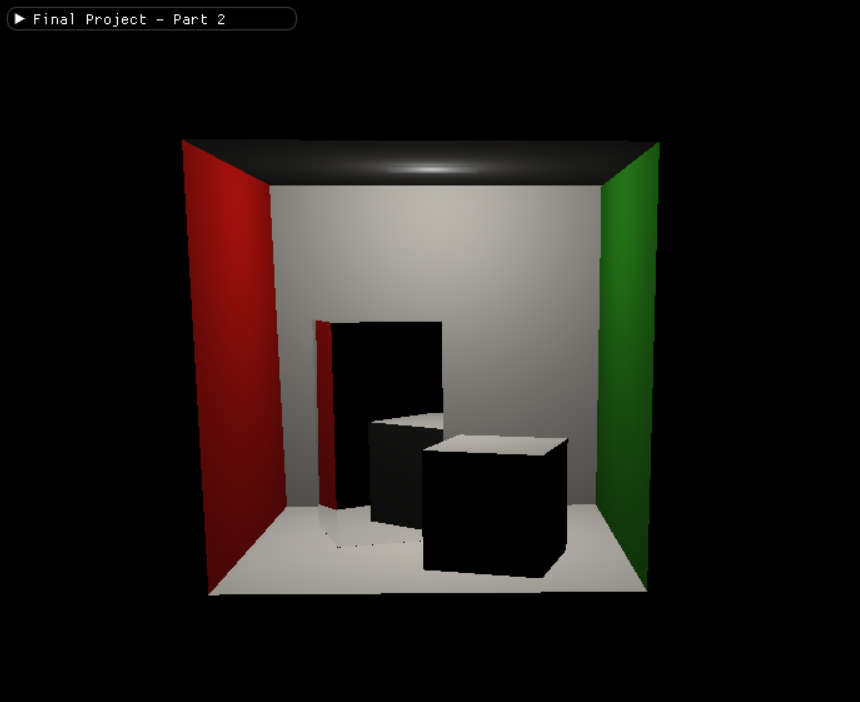
\includegraphics[scale=0.60]{images/recursive_ray_tracer_showcase.png}

        The complex specular effects produced by recursive ray tracing, which include proper mirror simulation

        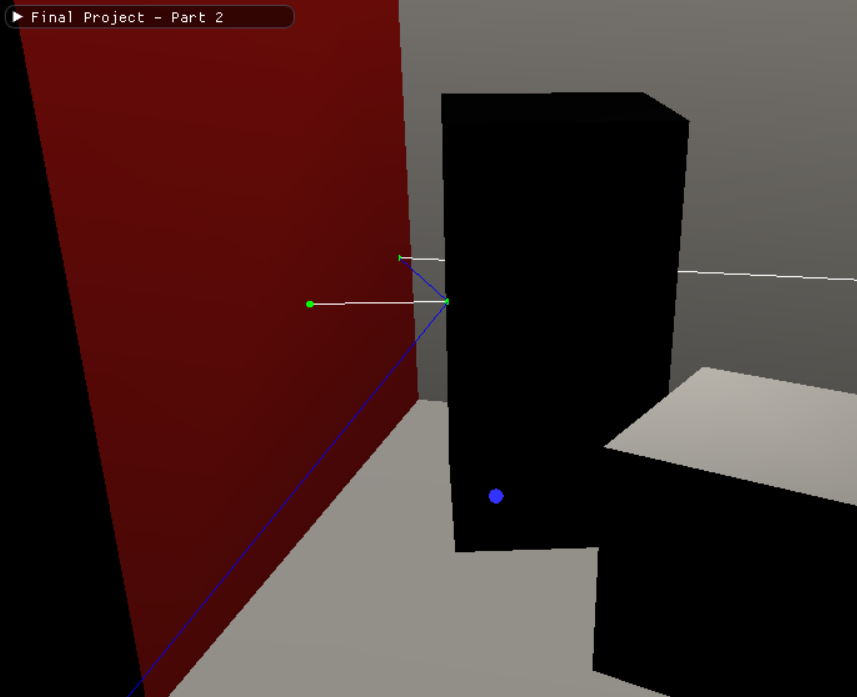
\includegraphics[scale=0.60]{images/recursive_ray_tracer_debug.png}

        The recursive ray tracer debug, showing two total rays in the recursive chain, along with their normals
    \end{center}

    \section{Models}
    To be constructed

    \section{Performance Test}
    To be constructed
\end{document}
